% This is samplepaper.tex, a sample chapter demonstrating the
% LLNCS macro package for Springer Computer Science proceedings;
% Version 2.20 of 2017/10/04
%
\documentclass[runningheads]{llncs}
%
\usepackage{graphicx}
\usepackage{amsmath}
\usepackage{algorithm} %format of the algorithm 
\usepackage{algorithmic} %format of the algorithm 
\usepackage{multirow} %multirow for format of table 
\usepackage{amsmath}
\usepackage{xcolor}
\renewcommand{\algorithmicrequire}{\textbf{Input:}} 
\renewcommand{\algorithmicensure}{\textbf{Output:}}

% Used for displaying a sample figure. If possible, figure files should
% be included in EPS format.
%
% If you use the hyperref package, please uncomment the following line
% to display URLs in blue roman font according to Springer's eBook style:
% \renewcommand\UrlFont{\color{blue}\rmfamily}

\begin{document}
%
\title{An New $k$-Nearest Neighbors Algorithm Considering Label Uncertainties of Training Samples}
%
%\titlerunning{Abbreviated paper title}
% If the paper title is too long for the running head, you can set
% an abbreviated paper title here
%
\author{Zhengfei Shen \and
Jian Cao }
%
\authorrunning{F. Author et al.}
% First names are abbreviated in the running head.
% If there are more than two authors, 'et al.' is used.
%
\institute{Shanghai Jiao Tong University, Shanghai, China }
%
\maketitle              % typeset the header of the contribution
%
\begin{abstract}
As a regular non-parametric method used for classification, the $k$-nearest neighbors algorithm ($k$-NN) predicts an unlabeled object using the $k$ closest samples whose labels are already known. However, in some cases, the labels given to the samples are not definite or even correct. As a result, the accuracy of the predictions can be affected by the uncertainties the labels of the training samples. In order to improve the performance of $k$-NN when the labels of training samples are uncertain, we propose an new $k$-NN algorithm. In this algorithm, the uncertainties of labels are measured firstly. Then the prediction is made based on the uncertain labels of the $k$ closest samples based on Dempster-Shafer theory. In addition, we also introduce 2 methods to compute the optimal $k$ value. Experiments on a real-world dataset prove that our algorithm has a better performance comparing with other algorithms. 

\keywords{$k$-Nearest Neighbors Algorithm \and Uncertainty \and Dempster-Shafer Theory}
\end{abstract}
%
%
%
\section{Introduction}
% \subsection{A Subsection Sample}
Classification is the problem of identifying to which category or sub-population a new observation belongs, on the basis of a training set of data containing observations or instances whose category membership is known. In many domains, classification is a main task \cite{ref_article1}. In this task, the information and features of a sample can be formally and numerically represented as a vector $(x_1,x_2,...,x_n)$. In such a $n$-dimensional feature space, the main goal of classification is to estimate the label of a new unlabeled vector by considering the relationships between the labeled and unlabeled vectors. 

As a well known and widely used method, the $k$-nearest neighbors algorithm ($k$-NN) method, has been regarded as the most simple but effective method among many available classification methods such as bayesian method, support vector machine and neural networks. Due to its simplicity but good performance, the $k$-NN has been considered as a top-10 data-mining method~\cite{ref_article2}. Known as a supervised learning algorithm, its working mechanism is fairly easy to grasp: for a given object, $k$-NN tries to get the nearest $k$ samples in the training data set based on a specific distance metric, and then makes prediction according to the information of these samples.  Generally, the object can be classified by a plurality vote of its neighbors, with the object being assigned to the class most common among its $k$ nearest neighbors. In the past few decades, some researches are also carried on to replace the plurality vote method with other approaches, for instance, in ~\cite{ref_article3}~\cite{ref_article4}, an evidence $k$-NN based on the Dempster-Shafer Theory is proposed to extend the plurality vote method.

Generally speaking, there are two important issues in $k$-NN. The first is about the similarity and distance computation between vectors. Recently many different distance computation algorithms have been proposed. The second issue is about the selection of optimal value of $k$ for a given data set. The general $k$-NN simply assumes the whole data set shares a value for $k$, which is often not proper and inaccurate for a finite and non-uniformly distributed data set. Recently, many new methods have been proposed to find the value of $k$ in an adaptive and optimal way. Unfortunately, in all of these efforts, the uncertainty of the training data is neglected. As we know, the training dataset is composed of a group of labeled data samples. However, these labels could be imprecise or even incorrect even they are provided by experts. Since the label information of the $k$ neighbors will be combined to make the ultimate decision, the label uncertainties of samples are superimposed so that the accuracy of the $k$-NN will decrease to some extent. Fortunately, additional and available information can used to quantify the uncertainty of the label of the sample itself including ratings from users or votes of experts. For instance, Zhu et al.~\cite{ref_article9} described a real-world decision support system for multi-disciplinary treatment called MdtDSS, the core recommend system predict a new patient's therapeutic regimen based on the information of other patients. The ultimate therapy of a patient is voted by a group of doctors which reflect doctors' opinions. The vote from one doctor expresses if he/she approves the ultimate therapy of this patient. 

In this paper, we define a method to quantify the uncertainties of samples in the training dataset with extra information. Then, we fuse both the uncertainty and the label information as the evidence of that sample in the $k$ nearest neighbors. Then, as to combine all these evidences, we use Dempster-shafer theory to accumulate  all these evidences to decide which class a test sample belongs to. Finally, we propose two strategies to select the optimal value for $k$ for a specific object based on the combined evidences. We perform a series of experiments on a real-world dataset mentioned in ~\cite{ref_article9} to verify our method.

This paper is organized as follows. In section 2, we discuss related work on $k$-NN algorithms. In Section 3, we introduce the Dempster-shafer evidence theory. In Section 4, we present a modified evidence-theory based on the uncertainties of data samples and the 2 algorithms upon optimal $k$ value selection for this sample. Finally, in the Section 5, experiments and results are presented.


\section{Related Work}
In order to improve the performance of $k$-NN, various studies have been conducted in recent years.

Lin et al. ~\cite{ref_article5} propose a similarity computing method via fusing neighborhood information. In this method, both the Euclidean distance and the neighbor information are considered simultaneously, the two metrics are combined together to measure the similarity between samples. Yung-Kyun Noh et al.~\cite{ref_article6} propose a generative metric learning method to enhance the performance of $k$-NN algorithm. In order to select the optimal value for $k$ on a given dataset,  Nicolás García-Pedrajas et al. ~\cite{ref_article7} propose an algorithm to obtain local $k$ value with a simple and fast procedure. Zhang et al. ~\cite{ref_article8} propose to learn a correlation matrix to reconstruct test data points by training data to assign different $k$ values to different test data points. 

The plurality vote method is the simplest rule to combine the labels of $k$ nearest neighbors and it is based on the assumption that each of the $k$ nearest neighbors are equally important. In practice, the circumstances can be more complex. Intuitively, the closer the neighbor, the more possible that the unknown object will be in the class of this neighbor. In 1995, Thierry Denœux~\cite{ref_article3} defined the frame of discernment ~\cite{ref_article10} of a $k$-NN method, and used  the distance of samples to measure the mass function of one sample. Our work is an extension to his work. To replace the plurality vote rule, some researchers investigate relationships between the global and local probability distributions. For a small training dataset, Sunsern Cheamanunkul ~\cite{ref_article11} propose a simple $k$-NN rule that takes into account the labels of all of the neighbors, rather than just the most common label. In his approach, relative entropy is used to measure the relationship between the global and local probability distribution.

Unfortunately, the previous studies neglect the uncertainties of labels of training samples, which is the topic of this paper. 

\section{Preliminary}
\subsection{Dempster-Shafer theory}
As a generalization of the Bayesian theory of subjective probability, Dempster Shafer theory was proposed in 1976 in ~\cite{ref_article10}. It is a general framework for reasoning with uncertainty data. This theory provides a model to express known and unknown  of different sources directly, and the ability to combine all the evidences. It mainly contains 2 crucial steps: Basic Belief Assignment(BBA) and evidence combination.

In the first step, let $U$ represents a non-empty set of mutually exclusive and exhaustive propositions called the frame of decrement. The power set $2^{U}$ is all subsets of the set $U$, which includes both the empty set  and the entire set $U$. For the frame of discernment $U$, the function $m$:$2^{U}$ $\rightarrow$ [0,1] is a basic probability assignment (BPA) also called a mass function. This function satisfies the following two conditions: 
\begin{equation}
\begin{split}
&(1)\ m(\phi) = 0\\&(2)\ \sum_{A\subset U}m(A) = 1
\end{split}
\end{equation}
$m(A)$ indicates the degree of trust exactly in $A$. The subsets $A$ of $U$ where $m(A)$ $>$ 0 are called the focal elements of the belief function, and their union is called its core. The function $Bel$:$2^{u}$ $\rightarrow$ [0,1] is the belief function over $U$, is defined as the sum of all the masses of subsets:

\begin{equation}
Bel(A) = \sum_{B\subset A}m(B)
\end{equation}

Belief (usually denoted $Bel$) measures the strength of the evidence in favor of a proposition but not any of its subsets. It ranges from 0 (indicating no evidence) to 1 (denoting certainty). An important difference with probability theory is the sum of belief of a proposition and its negation not necessarily equals to 1. Hence, the remaining belief of $A$, called total ignorance, is the belief of the whole frame of discernment.

In the second step, Dempster Shafer defines a method to combine two or more mass assignments of the same frame of discernment in specific situations. To combine there assignments means to accumulate all evidences from all sources in one frame.This rule derives common shared beliefs among multiple sources and ignores all the conflicting (non-shared) beliefs through a normalization factor. 

Given $n$ mass functions $m_1$,$m_2$...$m_n$ on the same frame of discernment $U$, for arbitrary $A$  included in $U$, the combination rule is as follow:
\begin{equation}
\begin{split}
&\ m_{1,2,...,n}(\phi) = 0\\
&\ 
\begin{split}
m_{1,2,...,n}(A)  &\ =(m_1\oplus m_2 \oplus \cdots 
\oplus m_n)(A) \\
&\ = \frac{1}{K} \sum_{A_1 \cap A_2 \cap \cdots
\cap A_n} m_1(A_1) \cdot m_2(A_2) \cdots m_n(A_n)
\end{split}
\end{split}
\end{equation}
where:
\begin{equation}
\begin{split}
K &\ = \sum_{A_1 \cap A_2 \cap \cdots
\cap A_n \ne \phi} m_1(A_1) \cdot m_2(A_2) \cdots m_n(A_n) \\
&\ = 1 - \sum_{A_1 \cap A_2 \cap \cdots
\cap A_n = \phi} m_1(A_1) \cdot m_2(A_2) \cdots m_n(A_n) 
\end{split}
\end{equation}
the $K$ is called a Normalization factor that is a measure of the amount of conflicts among mass functions. 

\subsection{Dempster-Shafer Theory based $k$-NN}

Also known as the evidence-theory based $k$-NN (EKNN) , the Dempster-Shafer (DS) theory based $k$-NN was proposed by Thierry Denux ~\cite{ref_article3} in 1995. He first established the connection between the multidimensional vector space in the $k$-NN algorithm and the frame of discernment in DS evidence theory. In this approach, each neighbor of a pattern is considered as an evidence supporting some hypotheses about the class membership of that pattern. The BPAs are calculated for each of the $k$ nearest neighbors. The belief of each hypothesis is obtained by aggregating BPAs using Dempster’s rule of combination. The contributions can be summarized into 2 points: (1) A generalized way to compute the BPA value of the each $k$ nearest neighbor respectively based on the distance to the unlabeled data samples; (2) The application of the combination rule into the $k$-NN with a special form. Our work is also based on the DS evidence theory and the considerations of uncertainties of neighbors are an extension to Thierry's work which will be presented in this section.

In a classification problem, the training dataset can be regarded as a collection of $N$ $p$-dimensional training samples represented by $X=\{x^i=(x_1^i,...,x_p^i)|i=1,...,N\}$  , every sample in the data set belongs to one and only one class from $M$ classes $C=\{C_1,...,C_M\}$. In the very beginning, each sample in the training data is labeled a class in $C$ with a certain degree of uncertainty, which will be discussed in detail in the following section. The labeled data set can be represented as a binary relationship $(X, L)$, where $L$ is the set of labels, that can be used to classify new patterns.

In the Dempster-Shafer theory based $k$-NN, all possible class set $C$ makes up the frame of discernment, to predict the true label of a unlabeled pattern $x^s$ equals to assign it to one class in $C$.

For this unlabeled new pattern $x^s$, the $k$ neighbors based on a specific distance measurement make up a set $\Phi^s$. Each neighbor in $\Phi^s$ provides a piece of evidence whether $x^s$ belongs to a specific class $Cq$ in $C$, the negation of this piece of evidence is totally innocent, i.e. it doesn't refer to $C$ itself rather than any subsets of $C$. If we use mass function to represent this piece of evidence, we get the following relationship:
\begin{equation}
\begin{split}
&\ m^{s,i}( \{C_q\}) = \alpha_q
\\
&\ m^{s,i}(C) = 1-\alpha_q
\end{split}
\end{equation}
where $i=1,2,...,k$.
\begin{definition}
 $\alpha _q$ reflects how much the intensity is that the neighbor $x_i$ supports that the unlabeled pattern $x^s$ should be classified as $C_q$.
\end{definition}
According to the definition 1, the $\alpha _q$ should be a function of distance from $x_i$ to $x_s$, because the smaller the distance between  $x_i$ and $x_s$ is,  the more crucial it is to decide whether the class of $x_s$ is the same with the class of $x_i$. Moreover, as the distance between $x_s$ and $x_i$ gets infinitely large, the belief function given by $m^{s,i}$ makes no sense, which means that one’s belief concerning the class of $x_s$ is no longer affected by one’s knowledge of the class of $x_i$.

we can replace $\alpha _q$ with any reasonable decreasing function $t$, here we use the following one:
\begin{equation}
\alpha_q (d^{s,i})= \alpha_0 e^{- d^{s,i} {\beta}}
\end{equation}
Then we can get all the $k$ mass functions of the $k$ nearest neighbors respectively so that the distance to $x_s$ is available. To make the ultimate decision which class $x_s$ belongs to, we should first combine all these pieces of evidence together based on the DS evidence combination rule. According to equation (3), for each class $q$, we get:
\begin{equation}
\begin{split}
&\ m^{s} _q( \{C_q\}) = 1- \prod_{x^i\in \Phi^s _q } (1-\alpha_q(d^{s,i}))
\\
&\ m^{s} _q(C) = \prod_{x^i\in \Phi^s _q } (1-\alpha_q(d^{s,i}))
\end{split}
\end{equation}

Notice that here the BPA function $m^s_q (\{ C_q \})$ measures the combined belief according to all the neighbors whose class is $C_q$.

Combining all the BPAs $m^s_q$ for each class, a global BPA $m^s=\oplus ^M _{q=1} m^s_q$ is obtained as:

\begin{equation}
\begin{split}
&\ m^{s} ( \{C_q\}) = \frac{m^{s}_q ( \{C_q\})
\prod_{r\neq q} m^s_r(C)}{K}
\\
&\ m^{s} ( C) = \frac{
\prod_{q=1} ^M m^s_q(C)}{K}
\end{split}
\end{equation}
where $K$ is the normalizing factor $q=1,2,..,M$.

In the last step of the evidence rule based $k$-NN, for each $C_q$ in $C$ we compute its BPA according to equation (8), and then assign $x_s$ with the optimal class. 

\section{Uncertainty and Evidence Theory based $k$-NN Algorithm (UCEkNN)}

In this section, we present our own $k$-NN algorithm based on uncertainty and evidence theory (UCEkNN), and then we proposed 2 optimal $k$ value selection algorithm based on the UCEkNN.

\subsection{UCEkNN}
According to equation (5), till now we use $\alpha _q$ to represent the BPA of one neighbor $x^i$ among $k$ nearest neighbors set whose class is $C_q$. In practice, however, there is some uncertainty of the label itself. While the BPA of each neighbor is combined, the uncertainties are also accumulated, and the accuracy of the ultimate prediction will decrease to some extent. From this prospective, the uncertainty of the label can not be ignored and we denote the uncertainty as $UC$:
\begin{definition}
 $UC^i$ whose value ranges from 0 to 1 describes the uncertainty of the label itself of the neighbor $x^i$ among the k nearest neighbors of $x^s$. $UC^i$ is depended and only depended by the neighbor's characteristics.
\end{definition}
According to definition 2 and equation 5, we propose a new form of the BPA function:
\begin{equation}
\begin{split}
&\ m^{s,i}( \{C_q\}) = \alpha_q \cdot {UC}^i
\\
&\ m^{s,i}(C) = 1-\alpha_q \cdot {UC}^i
\end{split}
\end{equation}

Similarly, according to DS combination rule, for each class $q$:
\begin{equation}
\begin{split}
&\ m^{s} _q( \{C_q\}) = 1- \prod_{x^i\in \Phi^s _q } (1-\alpha_q(d^{s,i} )\cdot UC^i)
\\
&\ m^{s} _q(C) = \prod_{x^i\in \Phi^s _q } (1-\alpha_q(d^{s,i} )\cdot UC^i)
\end{split}
\end{equation}
Although $UC^i$ has been discussed in ~\cite{ref_article3} as the imperfect labeling, our approach is intrinsically different. In our approach, we do not change the basic form of equation (5), i.e. we assume one neighbor only belongs  to one specific class in spite of uncertainty rather than two or more possible classes. Moreover,  we think $UC^i$ is independent of the distance, and can be accessed easily with some extra information of $x^i$. Here we use an opinion set to describe the extra information, we denote it as $OpS$:
\begin{definition}
 $OpS^i$ describes the extra information set of $x^i$, it can be a set of votes information, ratings information, or other reasonable information which illustrate experts' or users' subjective opinions on whether $x^i$ should be labeled with $C_q$.
\end{definition}
In practical applications, for the $k$-NN, the label of each sample is decided by a group of people, usually by experts. $OpS^i$ is such a set which contains the opinions. $OpS$ is accessible in many problems. For example, ~\cite{ref_article9} introduces a medical therapy recommendation system based on $k$-NN algorithm, for each patient in the training data set,  the ultimate therapy is voted by at least 5 doctors. The most voted therapy is used to label this patient. Here, the vote results of doctors' make up the $OpS$ of this patient.

Intuitively, the consistency of doctors' opinions reflects the complexity of making decisions. If all doctors vote to the same therapy, the case of that patient is not complex and it is easy to make a decision, while for the situation that there are different votes, the case of that patient can be sophisticated and controversial. 

We use the information entropy(IE) ~\cite{ref_article12} of $OpS^i$ to quantify its consistency:

\begin{equation}
H(OpS^i) =- \sum_{c \in C} P_{ic} \cdot log (P_{ic})
\end{equation}
where $P_ic$ is the proportion of class $c$ in $OpS^i$.

Moreover, the uncertainty $UC^i$ of the label of $x_i$ has some connections with the uncertainty of $OpS^i$. For a high-consistent case where $H(OpS^i)$ has a small value, the $UC^i$ should be more close to 1 while for a controversial case where $H(OpS^i)$ has a large value, the $UC^i$ should be more close to 0. From this prospective, we conclude the $UC^i$ is a decrease function of $H(OpS^i)$. We suggest to chose the following function:

\begin{equation}
UC^i=UC_0e^{-H(OpS^i)\beta_u}
\end{equation}

For a query instance of unknown category $x^s$, the prediction process is shown in Algorithm 1.


\begin{algorithm} %算法开始 
\caption{Outline of the proposed Algorithm} %算法的题目 
\label{alg1} %算法的标签 
\begin{algorithmic}[1] %此处的[1]控制一下算法中的每句前面都有标号 
\REQUIRE  a training set $T=\{(x_1,y_1),...,(x_n,y_n)\}, x_i \in \Re ^p$,  a reasonable k, a query instance $x^s$, $OpS^i$ for each sample in training set %输入条件(此处的REQUIRE默认关键字为Require,在上面已自定义为Input) 
\ENSURE the optimal label of $x^s$ %输出结果(此处的ENSURE默认关键字为Ensure在上面已自定义为Output) 
% if-then-else 
\STATE get the k  nearest neighbors set $N=\{(x_1,y_1),...,(x_k,y_k)\}, x_i \in \Re ^p$
% for loop 
\FORALL{$x^i$ in T}
\STATE calculate H($OpS^i$) for each $x^i$ using equation (11)
\STATE  calculate BPA for each $x^i$ using equation (9)
\ENDFOR
\FORALL{classification $C_q$ in C}
\STATE  calculate combining BPA ms($\{C_q\}$) of $C_q$
\ENDFOR
\STATE return the optimal label whose BPA ls the largest
\end{algorithmic}
\end{algorithm}
\subsection{Optimizing Values of $k$ for UCEkNN}
Traditional value selection algorithms for $k$ aim to find the global optimal $k$ for a fixed training data set and testing dataset. Although a good value might be obtained using cross validation (CV), the same value is unlikely to be optimal for the whole space spanned by the training set. In this brief, we devise a new greedy method for UCEkNN.

For different $k$ ranging in [$k_min$,$k_max$], the neighbor set of $x^s$ is different, so is the BPA of different classification. Consequently, to search an optimal $k$ for a unlabeled object is tantamount to determine the best opportunity when the BPA of all classifications meet some optimal conditions. Here, we provide two available conditions: 
\subsubsection{Condition 1}
For different $k$, the largest value of $ms(\{C_q\})$ reaches the maximum.
\subsubsection{Condition 2}
For different $k$, the difference between the largest and second largest value of $ms(\{C_q\})$ reaches the maximum.

Detailed execution steps of our approach under condition 1 and condition 2 are illustrated by Algorithm 2 and Algorithm 3 respectively.
\begin{algorithm} %算法开始 
\caption{Algorithm for Condition 1} %算法的题目 
\label{alg1} %算法的标签 
\begin{algorithmic}[1] %此处的[1]控制一下算法中的每句前面都有标号 
\REQUIRE  a training set $T=\{(x_1,y_1),...,(x_n,y_n)\}, x_i \in \Re ^p$,  a reasonable $k$, a query instance $x^s$, $OpS^i$ for each sample in the training set %输入条件(此处的REQUIRE默认关键字为Require,在上面已自定义为Input) 
\ENSURE the optimal label of $x^s$ %输出结果(此处的ENSURE默认关键字为Ensure在上面已自定义为Output) 
\FORALL{$k$ in [$k_{min}$,$k_{max}$]}
    \FORALL{classify $x^i$ in $T$}
    \STATE  calculate $H(OpS^i)$ for each $x^i$ using equation (11)
    \STATE  calculate BPA for each $x^i$ using equation (9)
    \ENDFOR
    \FORALL{classify $C_q$ in $C$}
    \STATE calculate combining BPA ms($\{C_q\}$) of $C_q$
    \ENDFOR
    \STATE get $m^s(A)=max\{m^s(\{C_q\}),C_q \in C\}$
\ENDFOR
\STATE return the optimal label whose BPA ls the largest
\end{algorithmic}
\end{algorithm}
\begin{algorithm} %算法开始 
\caption{Algorithm for Condition 2} %算法的题目 
\label{alg1} %算法的标签 
\begin{algorithmic}[1] %此处的[1]控制一下算法中的每句前面都有标号 
\REQUIRE  a training set $T=\{(x_1,y_1),...,(x_n,y_n)\}, x_i \in \Re ^p$,  a reasonable $k$, a query instance $x^s$, $OpS^i$ for each sample in training set %输入条件(此处的REQUIRE默认关键字为Require,在上面已自定义为Input) 
\ENSURE the optimal label of $x^s$ %输出结果(此处的ENSURE默认关键字为Ensure在上面已自定义为Output) 
\FORALL{$k$ in [$k_{min}$,$k_{max}$]}
    \FORALL{classify $x^i$ in $T$}
    \STATE  calculate H($OpS^i$) for each $x^i$ using equation (11)
    \STATE  calculate BPA for each $x^i$ using equation (9)
    \ENDFOR
    \FORALL{classify $C_q$ in $C$}
    \STATE calculate combining BPA $ms(\{C_q\})$ of $C_q$
    \ENDFOR
    \STATE get $m^s(A)=max\{m^s(\{C_q\}),C_q \in C\}$
    \STATE get $m^s(B)=max\{m^s(\{C_q\}),C_q \in C \ and \ C_q \ne A\}$
\ENDFOR
\STATE return the optimal label whose BPA is the largest
\end{algorithmic}
\end{algorithm}
\subsection{Optimization of UCEkNN Using $L$-Sure Algorithm}
Actually, the influences of the opinions about the data sample's label from different  experts or users should not be identical. For instance, in a medical decision, the opinion of an experienced and proficient doctor could be more crucial. From this prospective, just using entropy of $OpS$ to measure the uncertainty is not reasonable any more.

$L$-Sure algorithm is devised to intensify the opinions from more authoritative people who vote for the labels of a samples. The basic idea of $L$-Sure algorithm can be described as two steps: (1) to select $L$ most authoritative experts out of the vote set. (2) to calculate the uncertainty based on the opinions of these $L$ experts.
Given an unlabeled sample and its $k$ neighbors, a straightforward strategy to pick the $L$ most reliable experts is just sorting all the experts by the precision in the $k$ neighbors from high to low. Such a idea is easy but efficient.

After getting the $L$ experts for an unlabeled sample, the uncertainty can be calculated by the following conditions: (1) if all the $L$ experts hold the same opinion, then the $UC_i$ in equation (9) equals to 1; (2) if one or more experts out of $L$ experts hold different opinions, then we still use equation (12) to calculate the $UC^i$.

All the above steps can be described as equation (13):

\begin{equation}
UC^i=
\begin{cases}
UC_0& \text{condition 1}\\
UC_0e^{-H(OpS^i)\beta_u}& \text{condition 2}
\end{cases}
\end{equation}

\section{Experiments and Discussions}
\subsection{Experiments for UCEkNN and Optimal $k$ Values}
To testify our proposed two models (the original UCEkNN, UCEkNN with optimal $k$ values), we conduct two experiments which is \textbf{Experiment I} (for UCEkNN) and \textbf{Experiment II}(for UCEkNN with optimal $k$ values) using the same real-world data set in the MdtDSS mentioned in ~\cite{ref_article9}. The size of the dataset is 3340 if we only use it to examine the general kNN, however, only 1455 of them contain the voting information which can be used in our method. 

In the 1455 instances which have $OpS$, the average size of $OpS$ is 8 which means there are 8 doctors voting to one patient on average. We repeat the two experiments 3 times respectively based on 3 different subsets of the 1455 instances. Each of the subsets are divided into 3 segments which have different functions. The 3 segments are training data set, verification data set and testing data set. \textbf{Experiment I and II} use different part of the 3 segments: (1)\textbf{Experiment I} only uses the training data set; (2) \textbf{Experiment II} uses the training data set, verification data set and testing data set at the same time. The length of each segment during the 3 experiments is illustrated in Table 1.
\begin{table}
\begin{center}
\caption{Length of each segment during the 3 experiments.}\label{tab1}
\begin{tabular}{|c|c|c|c|}
\hline
experiment &  training & verification & testing\\
\hline
1 & 1028 & 212 & 215\\
2 & 790 & 238 & 427\\
3 & 610 & 347 & 239\\
\hline
\end{tabular}    
\end{center}
\end{table}

In  \textbf{Experiment I}, we predict the label of each instance in the testing data set using two methods: (1) the ordinary DS evidence rule based $k$-NN (EkNN), and (2) our proposed uncertainty based $k$-NN (UCEkNN). In this experiment, we use the globally optimal $k$ as the input of these two algorithms. We devise a simple greedy algorithm to select $k$ in [$k_{min}$,$k_{max}$]. We compare the predicted result and the actual result to judge if the prediction is correct, at last we calculate the accuracy of this experiment. The results of these 3 experiments are shown in Table 2.

\begin{table}
\begin{center}
\caption{Comparison Results of EkNN and UCEkNN }\label{tab1}
\begin{tabular}{|c|c|c|}
\hline
Experiment &  EkNN & UCEkNN\\
\hline
1 & 59.53\% & 66.05\%\\
2 & 63.00\% & 66.04\% \\
3 & 58.16\% & 64.01\%\\
\hline
\end{tabular}    
\end{center}
\end{table}

In \textbf{Experiment II}, we compare the performances of UCEkNN with different $k$ and with a fixed globally optimal $k$. Thus, we use (1) the fixed globally optimal $k$, (2) different $k$ acquired by the Algorithm 2 or (3) different $k$ acquired by the Algorithm 3 to predict the label of each instance in testing data set based on UCEkNN and compute the accuracy. The results are shown in Table 3.
\begin{table}
\begin{center}
\caption{Comparative Results of UcEkNN with Different Strategies to Select $k$}\label{tab1}
\begin{tabular}{|c|c|c|c|}
\hline
experiment &  fixed $k$ & diff $k$ based on Alg.1 & diff $k$ based on Alg.2\\
\hline
1 & 66.05\% & 70.70\%& 69.30\%\\
2 & 66.04\% & 69.79\%& 69.09\% \\
3 & 64.01\% & 67.36\%& 67.78\%\\
\hline
\end{tabular}    
\end{center}
\end{table}


in the \textbf{Experiment II}, an unlabeled object gets its label then becomes a historical instance and turns into a part of the training set. It is inflexible and inadvisable to keep a fixed $k$ nor calculate a new optimal $k$ at a regular interval. In contrast, our proposed method get a better performance in the accuracy.

\subsection{Experiments of L-Sure Algorithm}
To verify the efficiency of L-Sure algorithm and intensify the comparison against the normal UCEkNN algorithm, we conduct an experiment using the same data set with experiment 2,    and the capacity of the training, verification, and testing data set is  610,347,239 respectively. In our experiment, the value of L varies in the range of 0 to 16, and the result is shown in  \figurename{fig1}:

\begin{figure}
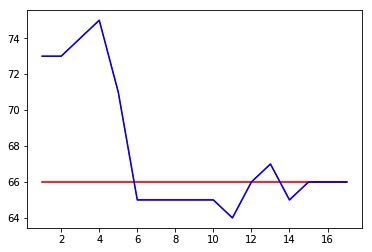
\includegraphics[width=\textwidth]{fig.jpg}
\caption{The red curve represents the normal UCEkNN while the blue curve represents UCEkNN with L-Sure algorithm. This figure shows that when L meets 6 to 11, the error times is lower than that without using L-Sure algorithm.} 
\label{fig1}
\end{figure}

\section{Conclusions}


\begin{thebibliography}{8}
\bibitem{ref_article1}
Zhu, Xiaofeng , X. Li , and S. Zhang . "Block-Row Sparse Multiview Multilabel Learning for Image Classification." IEEE TRANSACTIONS ON CYBERNETICS 46.2(2016):450.

\bibitem{ref_article2}
Wu, Xindong , et al. "Top 10 algorithms in data mining." Knowledge and Information Systems 14.1(2008):1-37.

\bibitem{ref_article3}
Denoeux, Thierry . "A k-nearest neighbor classification rule based on Dempster-Shafer theory." Systems Man \& Cybernetics IEEE Transactions on 25.5(1995):804-813.

\bibitem{ref_article4}
Wang, Lei , L. Khan , and B. Thuraisingham . "An Effective Evidence Theory Based K-Nearest Neighbor (KNN) Classification." 2008 IEEE/WIC/ACM International Conference on Web Intelligence and Intelligent Agent Technology IEEE, 2009.

\bibitem{ref_article5}
Lin, Yaojin , et al. "A new nearest neighbor classifier via fusing neighborhood information." Neurocomputing 143(2014):164-169.

\bibitem{ref_article6}
Noh, Yung Kyun , B. T. Zhang , and D. D. Lee . "Generative Local Metric Learning for Nearest Neighbor Classification." IEEE Trans Pattern Anal Mach Intell PP.99(2018):106-118.

\bibitem{ref_article7}
Garciapedrajas, Nicolas , J. A. R. Del Castillo , and G. Cerruelagarcia . "A Proposal for Local k Values for k-Nearest Neighbor Rule." IEEE Transactions on Neural Networks \& Learning Systems 28.2(2015):470.

\bibitem{ref_article8}
Zhang, Shichao , et al. "Learning k for kNN Classification." ACM Transactions on Intelligent Systems and Technology 8.3(2017):1-19. 

\bibitem{ref_article9}
Zhang, Yan , et al. "A Multi-disciplinary Medical Treatment Decision Support System with intelligent treatment recommendation." IEEE International Conference on Computer \& Communications IEEE, 2017.

\bibitem{ref_article10}
Rota, Gian Carlo . "297 ppG. Shafer, A Mathematical Theory of Evidence, Princeton University Press (1976). " Ade Bulletin 2(1977):N/A.

\bibitem{ref_article11}
Cheamanunkul, S , and Y. Freund . "Improved kNN Rule for Small Training Sets." International Conference on Machine Learning \& Applications IEEE, 2014.

\bibitem{ref_article12}
R Grey. Entropy and Information Theory. ENTROPY AND INFORMATION THEORY. 2012.


\end{thebibliography}
\end{document}
